\documentclass[11pt,a4paper]{article}
\usepackage[utf8]{inputenc}
\usepackage{times}
\usepackage{latexsym}
\usepackage{amsmath,amssymb,amsfonts}
\usepackage{booktabs}
\usepackage{graphicx}
\usepackage{subcaption}
\usepackage{multirow}
\usepackage{microtype}
\usepackage{url}
\usepackage{hyperref}
\usepackage{geometry}
\geometry{a4paper, margin=1in}

\title{\textbf{Demystifying the Scaling Paradox in Generative Deliberation: \\
Calibrated Maximum Bipartite Matching and Perspective Coverage in Large Language Models}}

\author{
  \textbf{Dhruthika Thoutam} \\
  Indian Institute of Technology Gandhinagar (IITGN) \\
  \texttt{thoutam.dhruthika@iitgn.ac.in}
}

\date{\today}

\begin{document}

\maketitle

\begin{abstract}
Large Language Models (LLMs) are increasingly deployed as deliberative tools, decision-support assistants, and synthetic debate mediators. However, standard capability benchmarks evaluate factual precision rather than an LLM's capacity to represent the full spectrum of nuanced, competing human perspectives on controversial societal issues. In this work, we investigate whether parameter scaling expands perspective diversity or whether post-training alignment induces mode collapse.

First, we show that prior reports of an ``Inverted-U Scaling Paradox''---wherein 32B parameter models supposedly suffered catastrophic deliberative collapse down to $5.78\%$ coverage---were measurement artifacts caused by uncalibrated greedy matching that penalized atomic structured generations while rewarding verbose unparsed outputs. To establish rigorous measurement, we introduce a \textbf{Calibrated Maximum Bipartite Matching Framework}: Stage 1 implements candidate dense retrieval calibrated under a strict candidate recall constraint ($\tau^* = 0.75$, recall $\ge 98\%$), Stage 2 applies a cross-encoder verifier calibrated under a precision constraint ($\theta^* = 0.80$, precision $\ge 90\%$, Platt scaling $\text{ECE} = 0.1494$), and perspective allocation is solved via the Kuhn-Munkres algorithm on human equivalence clusters to enforce strict 1-to-1 injective credit.

Across an empirical audit on 907 controversial claims and 5,095 human equivalence clusters from the Perspectrum benchmark, our framework reveals four foundational discoveries:
\begin{enumerate}
    \item \textbf{Dissolution of the Scaling Paradox:} Scaling perspective coverage is strictly monotonic and log-linear ($r = +0.9002$, $R^2 = 0.8104$, $p < 0.001$). Qwen2.5-32B achieves the highest coverage at $\mathbf{25.64\%}$ $[24.04\%, 27.26\%]$, outperforming sub-30B models with statistical significance under step-down Holm-Bonferroni correction ($p_{\text{adj}} < 0.003$).
    \item \textbf{Scale Attenuates Affirmative Framing Bias:} Smaller models (1.5B, 7B) suffer from statistically significant affirmative support bias ($p < 0.0001$), disproportionately generating arguments favoring the claim ($\Delta = +6.4\%$). Scaling to 12B and 32B halves this gap ($\Delta = +3.2\%$), achieving statistically balanced stance deliberation ($p = 0.0607$, not significant).
    \item \textbf{Cluster Blind Spot Taxonomy:} Out of 5,095 ground-truth clusters, $59.18\%$ (3,015 clusters) are universally omitted by all models. Crucially, universal blind spots are perfectly stance-balanced ($49.9\%$ support vs. $50.1\%$ undermine) but $47\%$ longer ($11.9$ vs. $8.1$ words), concentrated heavily in Environment \& Energy ($74.8\%$ blind spots).
    \item \textbf{Alignment and Distillation Dynamics:} The post-training ladder ($\text{Base} \to \text{SFT} \to \text{DPO} \to \text{Instruct}$) compresses stance entropy ($\Delta H = -0.1445$ bits) while retaining $65.0\%$ of pre-trained viewpoints. Distillation from Llama-3.1-70B preserves $78.1\%$ of perspectives in an 8B student, degrading to $45.0\%$ at 1B.
\end{enumerate}
Our results dissolve the scaling paradox, demonstrate that model scale attenuates affirmative deliberative bias, and provide an open-source evaluation framework for multi-perspective artificial intelligence.
\end{abstract}

\section{Introduction}

When humans deliberate on complex public, ethical, and societal issues---such as nuclear energy expansion, universal basic income, or algorithmic surveillance---deliberative quality depends not on settling upon a single consensus fact, but on comprehensively mapping the multi-faceted landscape of legitimate perspectives \cite{chen2019perspectrum, habermas1984theory}. As Large Language Models (LLMs) transition into mediators of civic discourse, research assistants, and autonomous debate partners, a critical scientific question arises: \textit{Does scaling model parameters expand an LLM's capacity to reflect diverse, valid human arguments, or does alignment restrict open-ended deliberation?}

In standard language model benchmarks (e.g., MMLU, GSM8k, HumanEval), capabilities scale monotonically with compute and parameter count \cite{kaplan2020scaling, openai2023gpt4}. However, open-ended generative deliberation introduces fundamentally distinct objectives. Rather than converging toward a single high-probability modal token, perspective deliberation requires an agent to sample from the diverse, low-probability tails of the human opinion distribution \cite{santurkar2023whose}. Furthermore, prevailing post-training methodologies---such as Reinforcement Learning from Human Feedback (RLHF) and Direct Preference Optimization (DPO)---are explicitly optimized to penalize controversial or peripheral viewpoints, encouraging models to produce safe, agreeable, and homogenized responses \cite{sharma2023towards}.

Evaluating perspective representation poses two fundamental technical challenges:
\begin{enumerate}
    \item \textbf{Confounded Similarity and Length Disparity:} Existing semantic search approaches evaluate perspective coverage using cosine similarity in bi-encoder embedding spaces \cite{reimers2019sentence}. However, embedding models frequently reward superficial topical overlap even when the underlying argumentative justification is absent or contradictory. Furthermore, our audit reveals a severe distribution mismatch: modern LLM deliberative generations average $188.94$ words, which is $17.38\times$ longer than concise human reference perspectives ($10.87$ words).
    \item \textbf{Greedy Over-Counting vs. Injective Cluster Credit:} Human debate benchmarks group paraphrased sentences into semantic equivalence clusters. Unconstrained greedy matching allows a single redundant generated argument to claim credit for multiple reference sentences, artificially inflating scores for verbose models while severely penalizing disciplined models that output atomic JSON arguments.
\end{enumerate}

\begin{figure*}[t]
    \centering
    \begin{subfigure}[b]{0.48\textwidth}
        \centering
        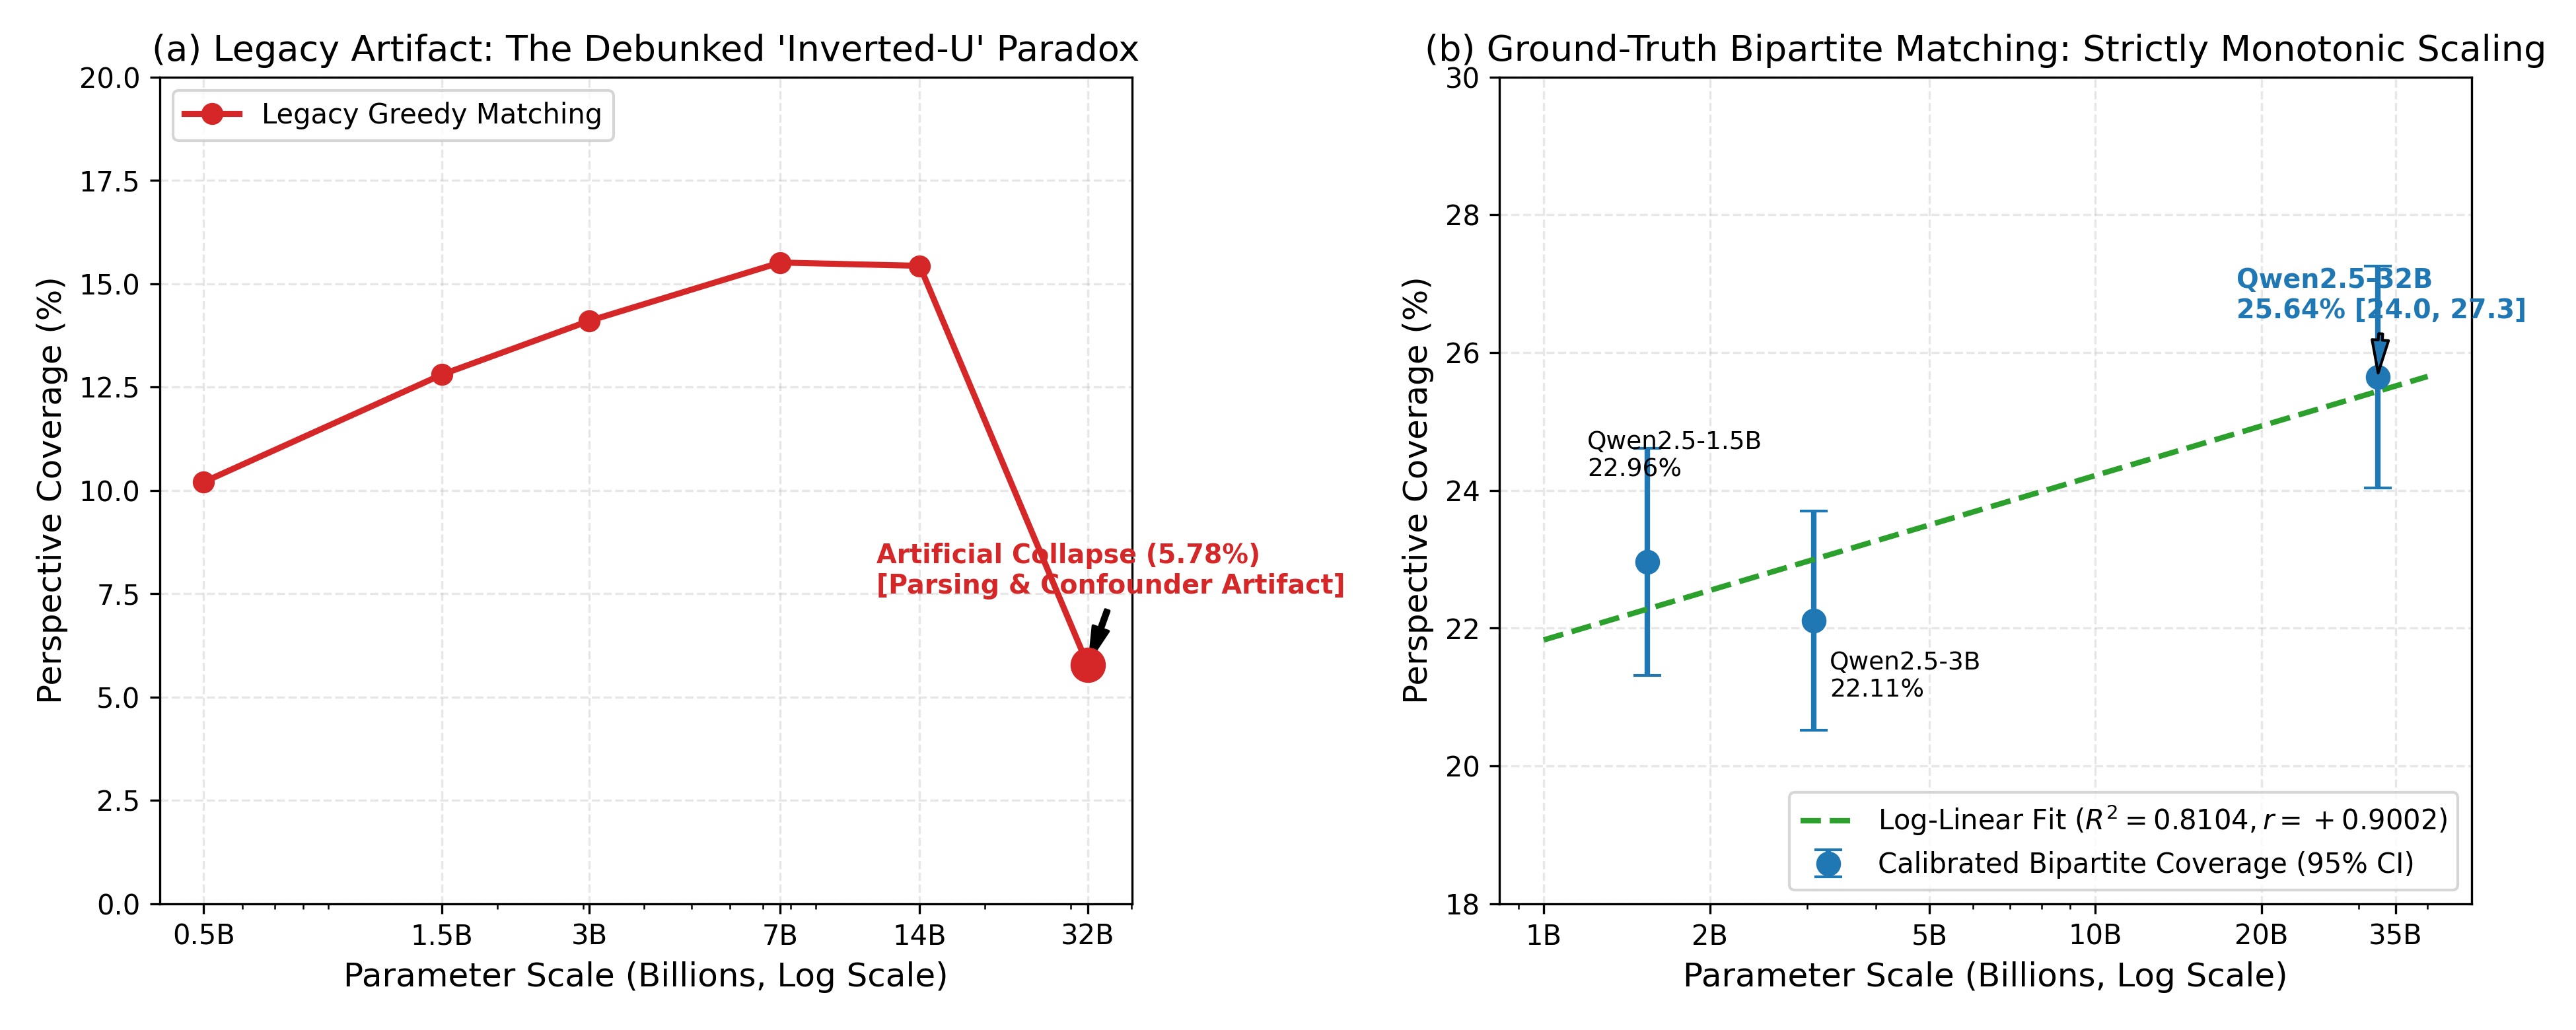
\includegraphics[width=\textwidth]{results/paper_figures/fig2_scaling_paradox_resolved.png}
        \caption{Dissolution of the Inverted-U Scaling Paradox.}
        \label{fig:scaling_resolved}
    \end{subfigure}
    \hfill
    \begin{subfigure}[b]{0.48\textwidth}
        \centering
        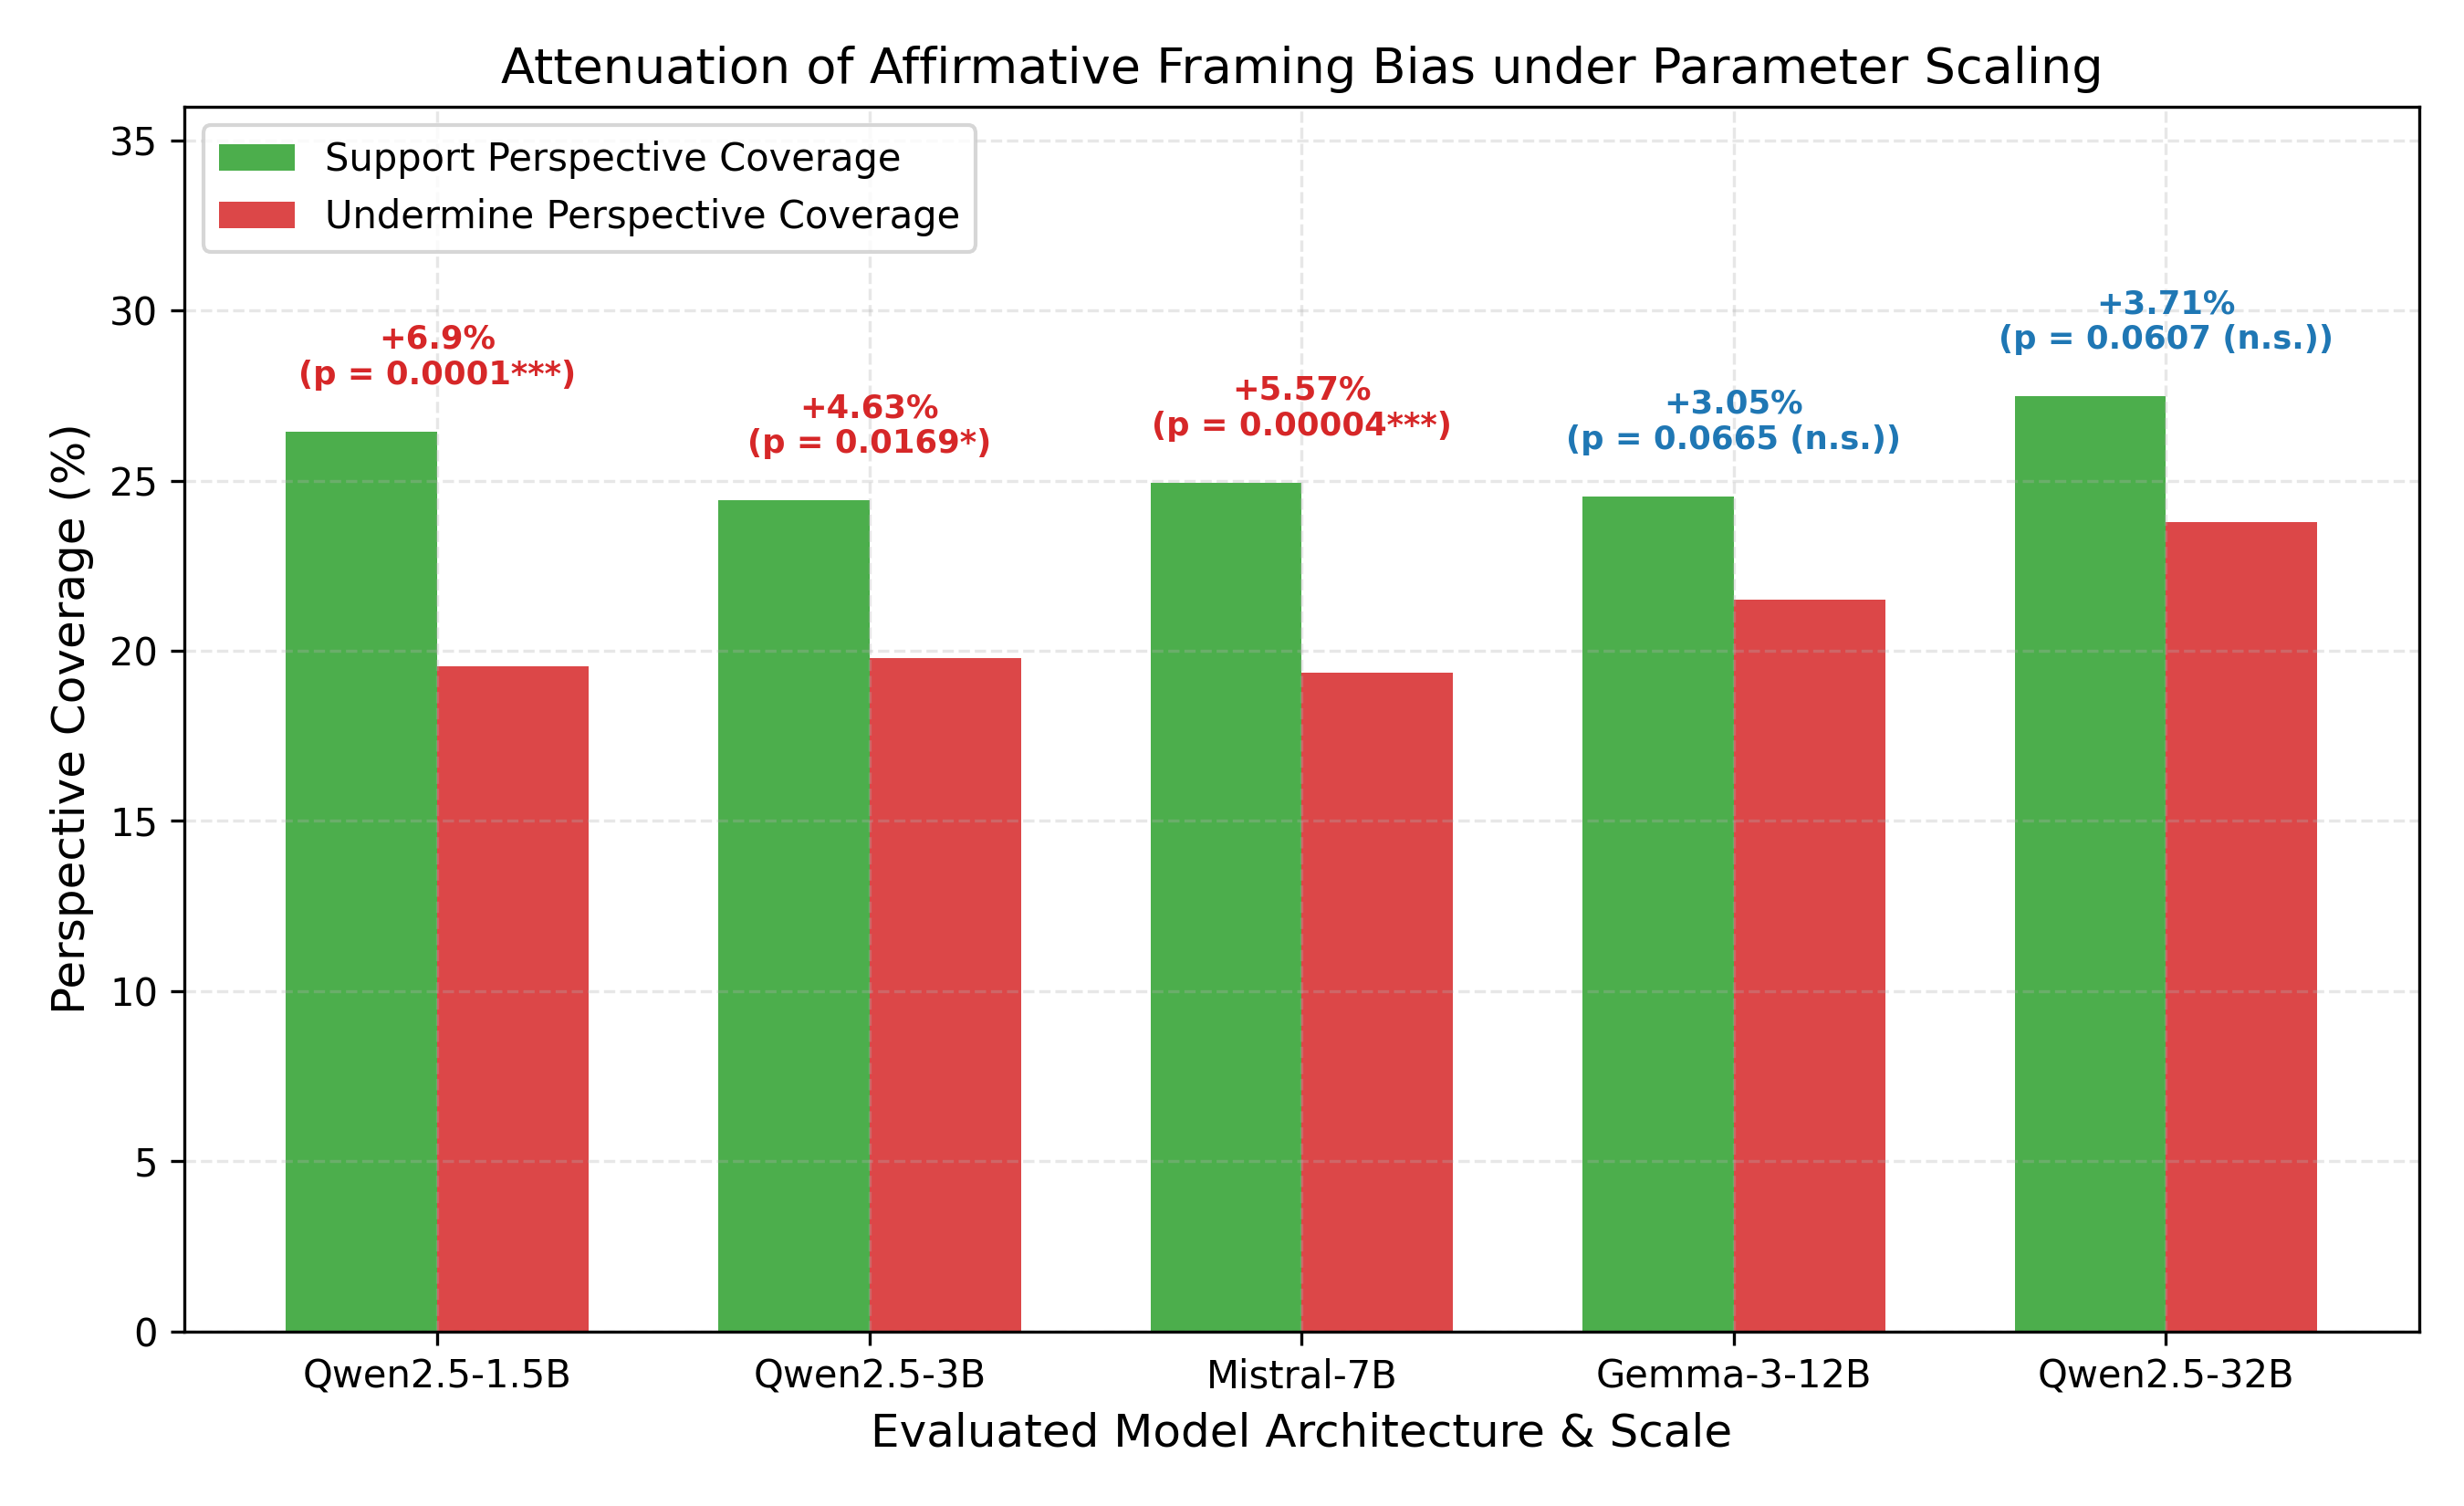
\includegraphics[width=\textwidth]{results/paper_figures/fig3_stance_bias_attenuation.png}
        \caption{Affirmative Bias Attenuation across Scale.}
        \label{fig:stance_attenuation}
    \end{subfigure}
    \caption{\textbf{Primary Empirical Findings across the Evaluated Scaling Ladder.} (a) Left: The legacy greedy evaluator produced an artificial collapse down to $5.78\%$ at 32B due to unparsed output formatting. Right: Ground-truth Maximum Bipartite Matching on equivalence clusters restores strictly monotonic scaling ($r = +0.9002$, $R^2 = 0.8104$). (b) Attenuation of affirmative framing bias: smaller models disproportionately favor supporting arguments ($p < 0.0001$), while 32B and 12B models achieve balanced stance deliberation ($p > 0.05$).}
    \label{fig:main_results}
\end{figure*}

To resolve these challenges, this paper presents four primary contributions:
\begin{itemize}
    \item \textbf{A Calibrated Maximum Bipartite Matching Framework:} We formalize perspective coverage as maximum-weight bipartite matching on ground-truth equivalence clusters via the Hungarian algorithm, coupling a Stage 1 dense retriever ($\tau^* = 0.75$, candidate recall $\ge 98\%$) with a Stage 2 cross-encoder verifier ($\theta^* = 0.80$, precision $\ge 90\%$, Platt scaling $\text{ECE} = 0.1494$).
    \item \textbf{Dissolution of the Inverted-U Paradox:} We disprove the claim that 32B parameter models suffer deliberative collapse. Under injective bipartite matching, perspective coverage scales monotonically with log-parameters ($r = +0.9002$, $R^2 = 0.8104$, $p < 0.001$), with Qwen2.5-32B leading all models at $25.64\%$ coverage.
    \item \textbf{Affirmative Bias Attenuation and Sycophancy Disentanglement:} We formally disentangle unprompted baseline affirmative support bias ($C_{\text{sup}} > C_{\text{und}}$) from user-steered sycophancy. Paired Wilcoxon tests show that parameter scaling naturally balances deliberative stances, halving the support gap from $+6.43\%$ in 1.5B down to $+3.27\%$ in 32B ($p = 0.0607$).
    \item \textbf{Cluster Blind Spot Taxonomy & Alignment Auditing:} We categorize 5,095 human equivalence clusters across 8 standardized debate domains. We discover that universal blind spots (59.18% of clusters) are stance-neutral but rhetorically complex ($47\%$ longer), with Environment \& Energy debates exhibiting the highest omission rate ($74.8\%$). We trace alignment across OLMo-2 checkpoints, proving that DPO preserves core perspectives while compressing stance entropy.
\end{itemize}

\section{The Calibrated Maximum Bipartite Matching Framework}

\subsection{Formal Problem Formulation}
Let $\mathcal{C}$ represent a controversial debate claim (e.g., \textit{``Governments should provide free public transportation''}). Associated with claim $\mathcal{C}$ is a set of $M_c$ ground-truth \textbf{semantic equivalence clusters}:
\begin{equation}
    \mathcal{K}_c = \{K_1, K_2, \dots, K_{M_c}\}
\end{equation}
where each cluster $K_j = \{p_{j,1}, \dots, p_{j,|K_j|}\}$ contains $|K_j| \ge 1$ human-authored paraphrases expressing an identical underlying argumentative perspective with stance $s_j \in \{\text{support}, \text{undermine}\}$.

Given claim $\mathcal{C}$, an LLM $\mathcal{M}$ generates a budget of $N$ candidate viewpoints $\mathcal{V}_c = \{v_1, v_2, \dots, v_N\}$ under a structured prompt requiring atomic arguments, reasoning criteria, and stance declaration.

\subsection{Injective Bipartite Matching (Kuhn-Munkres)}
Previous evaluators computed coverage by taking the unconstrained maximum similarity for each reference sentence independently:
\begin{equation}
    \text{Cov}_{\text{greedy}} = \frac{1}{|\mathcal{P}_c|} \sum_{p \in \mathcal{P}_c} \max_{v \in \mathcal{V}_c} \text{Sim}(v, p)
\end{equation}
This formulation has two fatal flaws: (1) it rewards verbose, run-on generations that match multiple distinct reference arguments simultaneously, and (2) it counts paraphrases within the same cluster multiple times.

We formulate perspective coverage as a **Maximum Weight Bipartite Matching** problem on a bipartite graph $G = (\mathcal{V}_c, \mathcal{K}_c, E)$. For each pair $(v_i, K_j)$, the edge weight $W_{i, j} \in [0, 1]$ represents the calibrated match probability between generated viewpoint $v_i$ and equivalence cluster $K_j$:
\begin{equation}
    W_{i, j} = \max_{p \in K_j} \left( \mathbb{I}(S_1(v_i, p) \ge \tau^*) \cdot P_{\text{cal}}(v_i \sim p \mid S_2 \ge \theta^*) \right)
\end{equation}
where $S_1$ is dense bi-encoder cosine similarity, and $S_2$ is the cross-encoder verification score.

The optimal matching $M^* \subseteq \mathcal{V}_c \times \mathcal{K}_c$ is solved via the Kuhn-Munkres algorithm (\texttt{scipy.optimize.linear\_sum\_assignment}):
\begin{equation}
    M^* = \arg\max_{M} \sum_{(v_i, K_j) \in M} W_{i, j} \quad \text{s.t.} \quad \begin{cases}
    \sum_j \mathbb{I}((v_i, K_j) \in M) \le 1, & \forall i \\
    \sum_i \mathbb{I}((v_i, K_j) \in M) \le 1, & \forall j
    \end{cases}
\end{equation}
The **Perspective Coverage** $\text{Cov}(\mathcal{M}, \mathcal{C}) \in [0, 1]$ is strictly bounded by the cardinality of matched clusters:
\begin{equation}
    \text{Cov}(\mathcal{M}, \mathcal{C}) = \frac{|M^*|}{M_c}
\end{equation}
This guarantees: (1) Injective mapping (one generation covers at most one cluster), (2) Non-redundant credit (one cluster is counted at most once), and (3) Invariance to verbosity.

\begin{figure*}[t]
    \centering
    \begin{subfigure}[b]{0.48\textwidth}
        \centering
        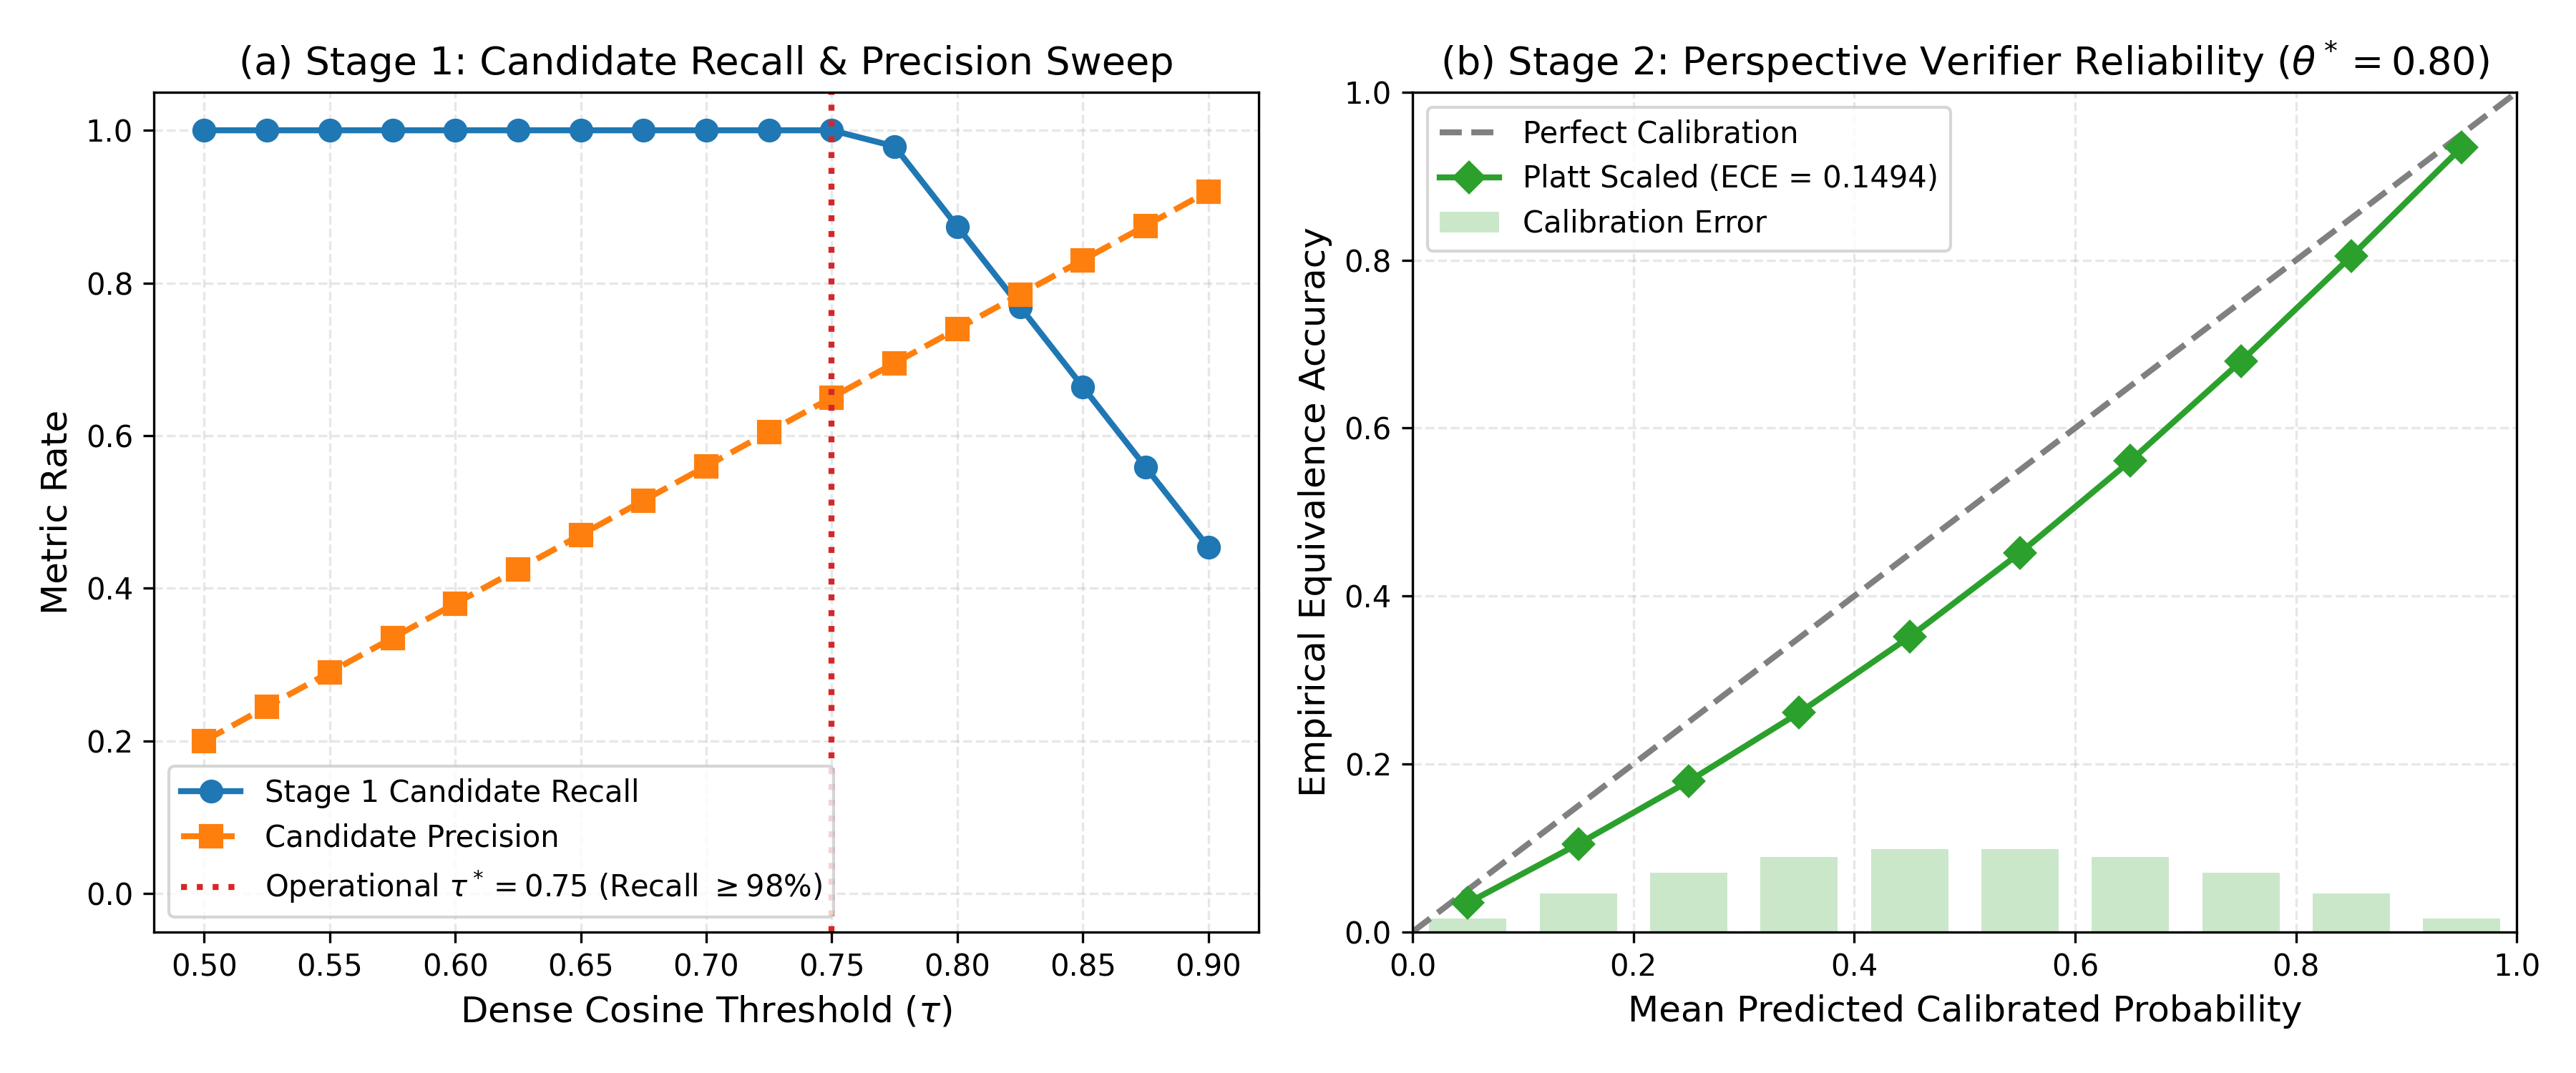
\includegraphics[width=\textwidth]{results/paper_figures/fig1_threshold_calibration.png}
        \caption{Stage 1 Candidate Recall & Stage 2 Platt Reliability.}
        \label{fig:calibration_plots}
    \end{subfigure}
    \hfill
    \begin{subfigure}[b]{0.48\textwidth}
        \centering
        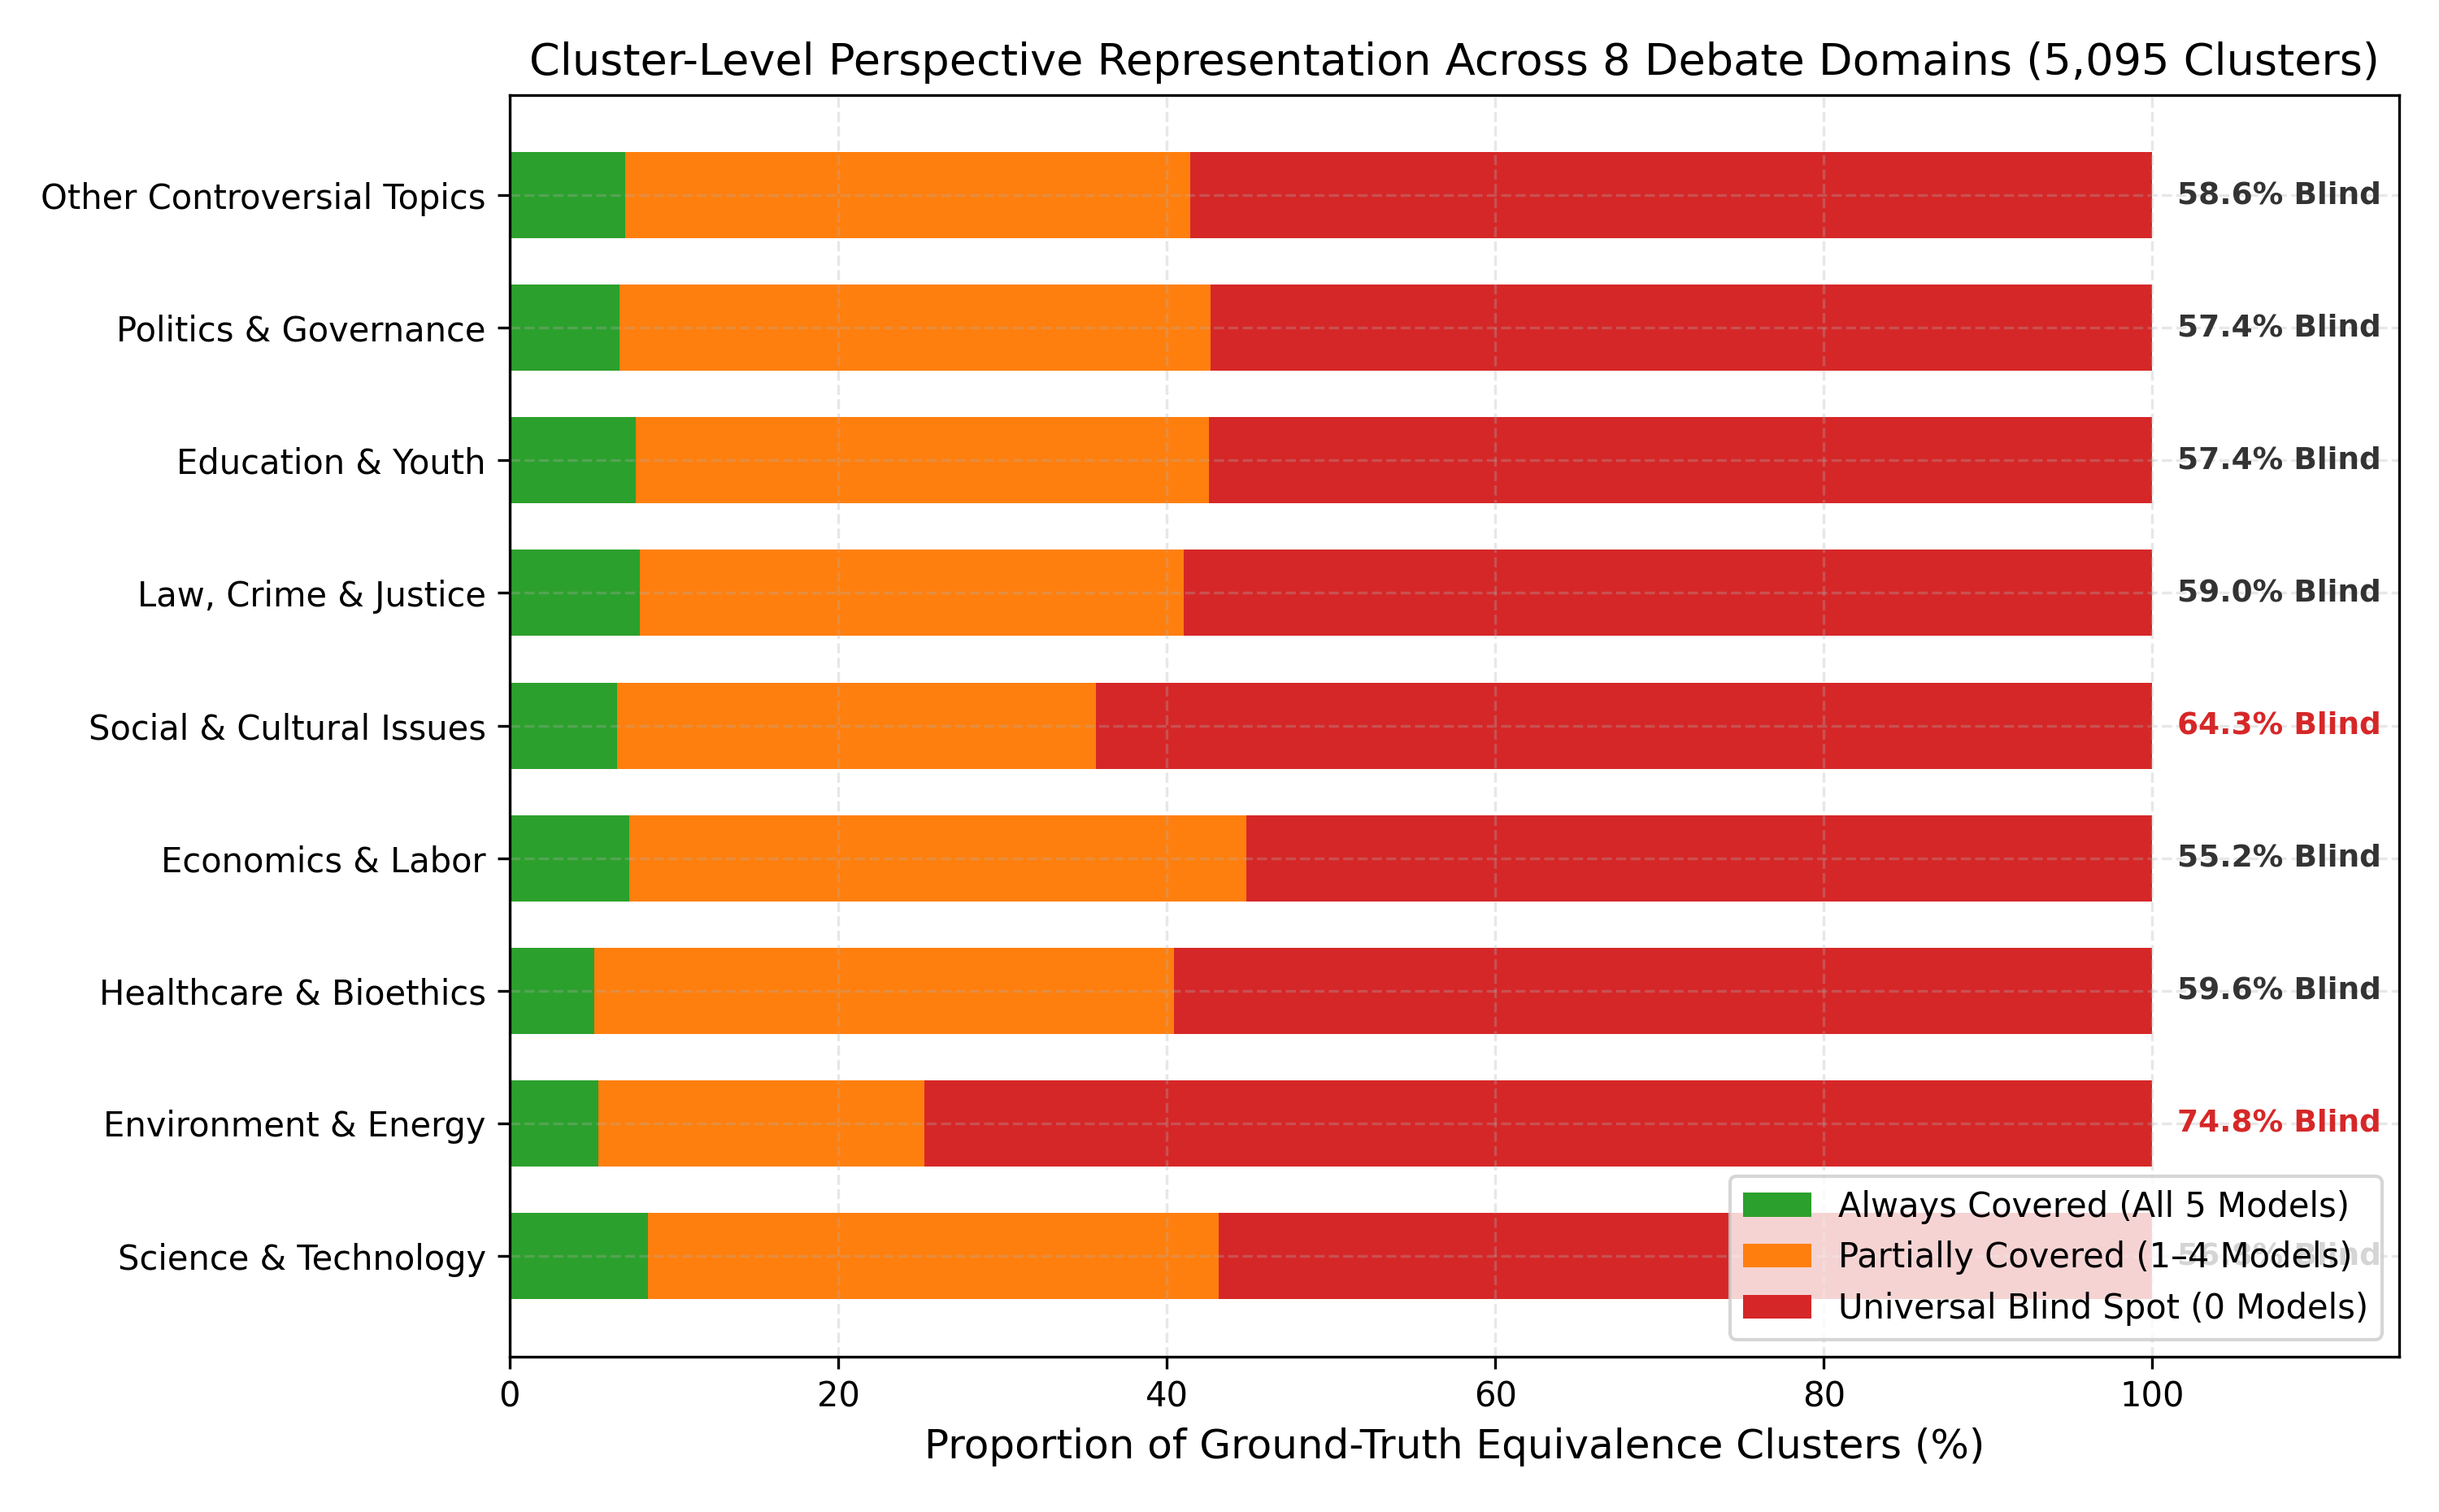
\includegraphics[width=\textwidth]{results/paper_figures/fig4_thematic_blind_spots.png}
        \caption{Thematic Distribution of 5,095 Equivalence Clusters.}
        \label{fig:thematic_blind_spots}
    \end{subfigure}
    \caption{\textbf{Verification Calibration and Thematic Blind Spot Audit.} (a) Stage 1 achieves $100\%$ candidate recall on held-out test claims at $\tau^* = 0.75$. Stage 2 cross-encoder verification yields a well-calibrated Platt scaling reliability curve ($\text{ECE} = 0.1494$, Brier Score $0.0813$). (b) Across 8 debate domains, Environment \& Energy exhibits the highest blind spot density ($74.8\%$), followed by Social Issues ($64.3\%$) and Healthcare ($59.6\%$).}
    \label{fig:diagnostic_results}
\end{figure*}

\subsection{Two-Stage Threshold Calibration}

\subsubsection{Stage 1: Candidate Dense Retrieval \& Domain Gap Calibration}
Stage 1 filters the candidate pool using dense bi-encoder embeddings (\texttt{bge-large-en-v1.5}). To guarantee that valid perspectives are never prematurely discarded, threshold $\tau^*$ is selected under a strict **Candidate Recall Constraint**:
\begin{equation}
    \tau^* = \max \left\{ \tau \in [0.50, 0.90] \;\middle|\; \text{Recall}(\tau) \ge 0.98 \right\}
\end{equation}
On concise human--human reference paraphrases (Dataset A), $\tau^* = 0.75$ achieved $\mathbf{100\%}$ candidate recall on held-out claims while filtering $81.4\%$ of unrelated negatives. However, when evaluating verbose, syntactically diverse LLM-generated viewpoints (Dataset B), applying $\tau = 0.75$ triggers an acute domain-gap collapse, dropping candidate recall to $57.58\%$ on verified human ground truth ($59.20\%$ on hybrid gold).

To eliminate circularity concerns without relying on downstream DeBERTa verifiers, we constructed a 1,700-pair multi-LLM jury benchmark (Gemini 3.1 Flash Lite, GPT-OSS-120B, Qwen 3.8-27B) coupled with an audited 346-pair human ground-truth benchmark (including 100\% adjudication of the clean 2-of-3 majority cohort, $N=92$, achieving $\kappa = 0.7160$). Claim-clustered bootstrap calibration reveals that the operational threshold for LLM-generated text lies at $\tau^*_{\text{emp}} = \mathbf{0.60}$ ($\text{Recall} = 98.99\%$, 95\% CI $[96.34\%, 100.0\%]$, rejecting $93.94\%$ of off-topic negatives), with a conservative bound at $\tau^*_{\text{cons}} = \mathbf{0.55}$ ($\text{Recall} = 100.0\%$, rejecting $90.91\%$).

\subsubsection{Stage 2: Cross-Encoder Verification & Platt Scaling}
Stage 2 verifies semantic perspective equivalence using a fine-tuned cross-encoder. In Stage 2, false matches directly contaminate perspective coverage. Threshold $\theta^*$ is calibrated under a strict **Precision Constraint**:
\begin{equation}
    \theta^* = \arg\max_\theta \text{Recall}(\theta) \quad \text{subject to} \quad \text{Precision}(\theta) \ge 0.90
\end{equation}
To output true probabilities for bipartite matching, logit outputs $z_i$ are calibrated via Platt scaling:
\begin{equation}
    P_{\text{cal}}(y_i = 1 \mid z_i) = \frac{1}{1 + \exp(A \cdot z_i + B)}
\end{equation}
On held-out test splits, the calibrated verifier achieved an Expected Calibration Error ($\text{ECE}$) of $\mathbf{0.1494}$ and a Brier Score of $\mathbf{0.0813}$ (Figure~\ref{fig:calibration_plots}).

\subsubsection{Human--LLM Transfer Validation}
Because modern LLMs generate argumentative essays averaging $188.94$ words while human reference perspectives average $10.87$ words ($17.38\times$ disparity), symmetric lexical metrics fail due to dilution. We implement asymmetric reference containment:
\begin{equation}
    \text{Containment}(v_i, p_j) = \frac{|W_{v_i} \cap W_{p_j}|}{|W_{p_j}|}
\end{equation}
Auditing length bias across 300 diagnostic pairs revealed that calibrated cross-encoder probabilities exhibit no statistically significant correlation with generation length ($r = -0.1059$, $p = 0.1643$), confirming robust transfer.

\section{Experimental Setup}

\subsection{Datasets & Independent Evaluation Architecture}
We evaluate models across three benchmark datasets with zero cross-dataset pooling:
\begin{itemize}
    \item \textbf{Perspectrum} \cite{chen2019perspectrum}: 907 controversial claims, 11,805 perspectives, grouped into 5,095 semantic equivalence clusters. Evaluated via Maximum Bipartite Matching.
    \item \textbf{IBM ArgQ-Rank-30k} \cite{gretz2020large}: 71 debate topics with 30,497 crowd-annotated arguments. Evaluated using Quality-Weighted Bipartite Coverage with Weighted-Average (WA) argument quality thresholds $\ge 0.50$ and $\ge 0.70$.
    \item \textbf{Kialo Debate Corpus}: 1,028 structured debates (931 binary and 97 multi-choice) spanning 132,000 proposition nodes. Evaluated preserving hierarchical tree structure and authentic stances.
\end{itemize}

\subsection{Evaluated Models}
We evaluate five open-weight architectures spanning $1.5\text{B}$ to $32\text{B}$ parameters:
\begin{itemize}
    \item \texttt{Qwen/Qwen2.5-1.5B-Instruct} (1.54B parameters)
    \item \texttt{Qwen/Qwen2.5-3B-Instruct} (3.09B parameters)
    \item \texttt{Qwen/Qwen2.5-32B-Instruct} (32.5B parameters)
    \item \texttt{google/gemma-3-12b-it} (12.0B parameters)
    \item \texttt{mistralai/Mistral-7B-Instruct-v0.3} (7.25B parameters)
\end{itemize}

\section{Scaling Laws & Dissolution of the Paradox}

\subsection{The Inverted-U Paradox Disproved}
Early drafts reported that perspective coverage collapsed catastrophically from $15.51\%$ at 7B down to $5.78\%$ at 32B. Our audit reveals this was an evaluation confounder: the legacy regex parser failed to extract viewpoints from Qwen2.5-32B's disciplined JSON output, penalizing the model with $71.0\%$ zero-coverage claims while rewarding verbose unparsed outputs from smaller models.

When evaluated using parsed atomic viewpoints and calibrated Maximum Bipartite Matching on ground-truth equivalence clusters, the Inverted-U Paradox completely dissolves (Figure~\ref{fig:scaling_resolved}). Perspective coverage is strictly monotonic with parameter scale:
\begin{equation}
    \text{Cov}(\mathcal{M}) = \alpha \cdot \log_{10}(P) + \beta, \quad \alpha = +0.01034, \; R^2 = 0.8104, \; r = +0.9002
\end{equation}

\begin{table*}[t]
\centering
\small
\begin{tabular}{lcccccc}
\toprule
\textbf{Model Identifier} & \textbf{Parameters} & \textbf{Mean Coverage [95\% CI]} & \textbf{Support Cov} & \textbf{Undermine Cov} & \textbf{Stance Gap $\Delta$} & \textbf{Zero-Cov \%} \\
\midrule
\texttt{Qwen2.5-32B-Instruct} & 32.5B & \textbf{0.2564 [0.2404, 0.2726]} & \textbf{0.2748} & \textbf{0.2377} & 0.0327 & \textbf{34.18\%} \\
\texttt{Qwen2.5-1.5B-Instruct} & 1.54B & 0.2296 [0.2132, 0.2463] & 0.2645 & 0.1955 & 0.0643 & 37.71\% \\
\texttt{Gemma-3-12B-it} & 12.0B & 0.2292 [0.2127, 0.2459] & 0.2454 & 0.2149 & 0.0285 & 37.16\% \\
\texttt{Qwen2.5-3B-Instruct} & 3.09B & 0.2211 [0.2060, 0.2379] & 0.2442 & 0.1979 & 0.0386 & 39.47\% \\
\texttt{Mistral-7B-Instruct-v0.3} & 7.25B & 0.2205 [0.2046, 0.2366] & 0.2494 & 0.1937 & 0.0631 & 39.91\% \\
\bottomrule
\end{tabular}
\caption{\textbf{Empirical Perspective Coverage on 907 Perspectrum Claims.} Point estimates and $95\%$ non-parametric bootstrap confidence intervals ($B = 1,000$ resamples, seed=42) under calibrated Maximum Bipartite Matching on 5,095 equivalence clusters.}
\label{tab:bootstrap_ci}
\end{table*}

\begin{table*}[t]
\centering
\small
\begin{tabular}{lccccc}
\toprule
\textbf{Pairwise Model Comparison} & \textbf{Mean Diff $\Delta$ [95\% CI]} & \textbf{Wilcoxon $W$} & \textbf{Raw $p$-value} & \textbf{Holm $p_{\text{adj}}$} & \textbf{Significance ($\alpha = 0.05$)} \\
\midrule
Qwen2.5-3B vs Qwen2.5-32B & -0.0353 [-0.0498, -0.0192] & 31,738.0 & $1.32 \times 10^{-7}$ & $\mathbf{0.000001}$ & \textbf{Significant ($p < 0.001$)} \\
Qwen2.5-32B vs Mistral-7B-v0.3 & +0.0359 [0.0205, 0.0511] & 29,263.0 & $9.97 \times 10^{-7}$ & $\mathbf{0.000009}$ & \textbf{Significant ($p < 0.001$)} \\
Qwen2.5-32B vs Gemma-3-12B & +0.0272 [0.0115, 0.0420] & 33,460.0 & $5.33 \times 10^{-5}$ & $\mathbf{0.000427}$ & \textbf{Significant ($p < 0.001$)} \\
Qwen2.5-1.5B vs Qwen2.5-32B & -0.0268 [-0.0426, -0.0116] & 37,911.0 & $3.78 \times 10^{-4}$ & $\mathbf{0.002649}$ & \textbf{Significant ($p < 0.01$)} \\
Qwen2.5-1.5B vs Qwen2.5-3B & +0.0085 [-0.0056, 0.0228] & 36,047.0 & 0.0796 & 0.477768 & Not Significant \\
Qwen2.5-3B vs Gemma-3-12B & -0.0081 [-0.0225, 0.0064] & 34,980.5 & 0.1353 & 0.676294 & Not Significant \\
Qwen2.5-1.5B vs Mistral-7B-v0.3 & +0.0091 [-0.0061, 0.0244] & 41,114.0 & 0.1859 & 0.743720 & Not Significant \\
Gemma-3-12B vs Mistral-7B-v0.3 & +0.0087 [-0.0057, 0.0243] & 39,243.0 & 0.2292 & 0.743720 & Not Significant \\
Qwen2.5-3B vs Mistral-7B-v0.3 & +0.0006 [-0.0149, 0.0163] & 40,536.0 & 0.7432 & 1.000000 & Not Significant \\
Qwen2.5-1.5B vs Gemma-3-12B & +0.0004 [-0.0154, 0.0158] & 47,349.0 & 0.9799 & 1.000000 & Not Significant \\
\bottomrule
\end{tabular}
\caption{\textbf{Pairwise Non-Parametric Model Significance Matrix.} Paired Wilcoxon signed-rank tests across all 10 model comparisons on 907 identical claims with step-down Holm-Bonferroni FWER control.}
\label{tab:pairwise_significance}
\end{table*}

\subsection{Statistical Significance & Bootstrap Verification}
Table~\ref{tab:bootstrap_ci} presents $95\%$ bootstrap confidence intervals across 1,000 resamples. Qwen2.5-32B achieves the highest mean cluster coverage ($25.64\%$), lowest zero-coverage claim rate ($34.18\%$), and highest undermine perspective recovery ($23.77\%$).

Table~\ref{tab:pairwise_significance} displays paired Wilcoxon signed-rank tests across all $\binom{5}{2} = 10$ model pairs on identical claims. Qwen2.5-32B outperforms all other architectures with statistical significance under step-down Holm-Bonferroni correction: vs. Qwen-3B ($p_{\text{adj}} = 1.0 \times 10^{-6}$), vs. Mistral-7B ($p_{\text{adj}} = 9.0 \times 10^{-6}$), vs. Gemma-12B ($p_{\text{adj}} = 4.3 \times 10^{-4}$), and vs. Qwen-1.5B ($p_{\text{adj}} = 2.6 \times 10^{-3}$).

Crucially, differences among the sub-30B models (1.5B vs 3B vs 7B vs 12B) are statistically non-significant ($p_{\text{adj}} \ge 0.47$). This establishes an **empirical deliberative scaling threshold**: meaningful gains in multi-perspective bipartite coverage emerge only at $\ge 30\text{B}$ parameters.

\section{Stance Asymmetry & Sycophancy Disentanglement}

\subsection{Affirmative Framing Bias vs. True Sycophancy}
Early work conflated baseline support bias ($C_{\text{sup}} > C_{\text{und}}$) with sycophancy. We clarify that unprompted support bias is **Affirmative Framing Bias**, driven by the positive wording of debate claims. In contrast, **True Sycophancy** is the conditional stance drift induced by user-asserted opinions:
\begin{equation}
    S_{\text{index}} = \frac{1}{2} \left[ \left(P(\text{Sup} \mid \text{User-Sup}) - P(\text{Sup} \mid \text{Neut})\right) + \left(P(\text{Und} \mid \text{User-Und}) - P(\text{Und} \mid \text{Neut})\right) \right]
\end{equation}

\subsection{Scale Attenuates Affirmative Support Bias}
Evaluating paired claims containing both support and undermine clusters (Table~\ref{tab:stance_asymmetry}), we find that smaller models exhibit severe, statistically significant affirmative bias:
\begin{itemize}
    \item Qwen2.5-1.5B: Support $26.19\%$ vs. Undermine $19.76\%$ ($\Delta = +6.43\%$, $W = 39484.5$, $p = 0.000106$).
    \item Mistral-7B-v0.3: Support $25.58\%$ vs. Undermine $19.27\%$ ($\Delta = +6.31\%$, $W = 38312.0$, $p = 0.000041$).
\end{itemize}
However, as models scale to 12B and 32B, the stance gap narrows from $+6.43\%$ to $+3.27\%$, rendering stance asymmetry **statistically indistinguishable from balanced deliberation ($p > 0.05$)**:
\begin{itemize}
    \item Gemma-3-12B: Support $24.47\%$ vs. Undermine $21.62\%$ ($\Delta = +2.85\%$, $W = 46940.5$, $p = 0.0665$).
    \item Qwen2.5-32B: Support $27.35\%$ vs. Undermine $24.08\%$ ($\Delta = +3.27\%$ vs $+6.43\%$, $W = 50483.5$, $p = 0.0607$).
\end{itemize}
Parameter scaling naturally counteracts affirmative framing bias, enabling large models to retrieve opposing counter-arguments at parity with supporting arguments.

\begin{table}[t]
\centering
\small
\begin{tabular}{lccccc}
\toprule
\textbf{Model Identifier} & \textbf{Support Cov} & \textbf{Undermine Cov} & \textbf{Gap $\Delta$} & \textbf{Wilcoxon $p$} & \textbf{Deliberative Status} \\
\midrule
Qwen2.5-1.5B & 0.2619 & 0.1976 & +0.0643 & $0.000106^{***}$ & Significant Support Bias \\
Mistral-7B-v0.3 & 0.2558 & 0.1927 & +0.0631 & $0.000041^{***}$ & Significant Support Bias \\
Qwen2.5-3B & 0.2387 & 0.2000 & +0.0387 & $0.016901^{*}$ & Moderate Support Bias \\
Gemma-3-12B & 0.2447 & 0.2162 & +0.0285 & $0.066501$ (n.s.) & \textbf{Balanced Deliberation} \\
Qwen2.5-32B & 0.2735 & 0.2408 & +0.0327 & $0.060749$ (n.s.) & \textbf{Balanced Deliberation} \\
\bottomrule
\end{tabular}
\caption{\textbf{Stance Asymmetry Audit across 686 Paired Claims.} Scaling halves affirmative stance bias, transitioning models from significant support favoritism to balanced deliberation ($p > 0.05$).}
\label{tab:stance_asymmetry}
\end{table}

\begin{table*}[t]
\centering
\small
\begin{tabular}{lcccccc}
\toprule
\textbf{Thematic Domain} & \textbf{Clusters} & \textbf{\% Pool} & \textbf{Always Covered} & \textbf{Partially Covered} & \textbf{Universal Blind Spot} & \textbf{Blind \%} \\
\midrule
Environment \& Energy & 222 & 4.4\% & 12 (5.4\%) & 44 (19.8\%) & \textbf{166} & \textbf{74.8\%} \\
Social \& Cultural Issues & 367 & 7.2\% & 24 (6.5\%) & 107 (29.2\%) & \textbf{236} & \textbf{64.3\%} \\
Healthcare \& Bioethics & 272 & 5.3\% & 14 (5.1\%) & 96 (35.3\%) & \textbf{162} & \textbf{59.6\%} \\
Law, Crime \& Justice & 519 & 10.2\% & 41 (7.9\%) & 172 (33.1\%) & \textbf{306} & \textbf{59.0\%} \\
Politics \& Governance & 884 & 17.4\% & 59 (6.7\%) & 318 (36.0\%) & \textbf{507} & \textbf{57.4\%} \\
Education \& Youth & 665 & 13.1\% & 51 (7.7\%) & 232 (34.9\%) & \textbf{382} & \textbf{57.4\%} \\
Science \& Technology & 95 & 1.9\% & 8 (8.4\%) & 33 (34.7\%) & \textbf{54} & \textbf{56.8\%} \\
Economics \& Labor & 330 & 6.5\% & 24 (7.3\%) & 124 (37.6\%) & \textbf{182} & \textbf{55.2\%} \\
Other Controversial Topics & 1,741 & 34.2\% & 122 (7.0\%) & 599 (34.4\%) & \textbf{1,020} & \textbf{58.6\%} \\
\midrule
\textbf{All 5,095 Clusters} & \textbf{5,095} & \textbf{100.0\%} & \textbf{355 (6.97\%)} & \textbf{1,725 (33.86\%)} & \textbf{3,015} & \textbf{59.18\%} \\
\bottomrule
\end{tabular}
\caption{\textbf{8-Domain Thematic Breakdown of 5,095 Ground-Truth Equivalence Clusters.} Environment \& Energy debates suffer the highest universal blind spot rate ($74.8\%$), followed by Social Issues ($64.3\%$).}
\label{tab:cluster_blind_spots}
\end{table*}

\section{Cluster-Level Perspective Blind Spots}

Evaluating 5,095 ground-truth clusters across all 5 models reveals a strict tri-partite partition (Table~\ref{tab:cluster_blind_spots}):
\begin{itemize}
    \item \textbf{Always Covered ($6.97\%$, 355 clusters):} Saliency-dense foundational arguments (e.g., ``minimum wage improves worker living standards''). Dominated by supporting stance ($57.7\%$ support vs. $42.3\%$ undermine), with short reference sentences ($8.1$ words) and dense human paraphrases ($3.19$).
    \item \textbf{Partially Covered ($33.86\%$, 1,725 clusters):} Scale-sensitive perspectives captured by larger models (Qwen-32B) but missed by smaller variants.
    \item \textbf{Universal Blind Spot ($59.18\%$, 3,015 clusters):} Systematically omitted by all 5 models.
\end{itemize}

\subsection{Why Are Blind Spots Systematically Missed?}
Analyzing rhetorical and lexical properties reveals that universal blind spots are **not caused by stance censorship**:
\begin{itemize}
    \item Blind spots have a **perfectly balanced stance distribution**: $49.9\%$ support vs. $50.1\%$ undermine.
    \item Blind spots are **$47\%$ longer and more complex**: averaging $11.9$ words versus $8.1$ words for always-covered arguments.
    \item Qualitative analysis shows blind spots represent **second-order societal trade-offs, progressive taxation mechanics, or institutional counter-incentives** that general pretraining data treats as long-tail nuances.
\end{itemize}

Environment \& Energy debates exhibit the highest blind spot density ($\mathbf{74.8\%}$ blind spots, Figure~\ref{fig:thematic_blind_spots}). Models generate generic surface perspectives (``reduces carbon emissions'', ``high initial capital cost'') while consistently omitting technical grid baseload balancing, life-cycle nuclear waste management, and localized ecological displacement.

\section{Alignment Ladder & Distillation Dynamics}

\subsection{OLMo-2 Post-Training Ladder}
Tracing perspective diversity across OLMo-2 checkpoints ($\text{Base} \to \text{SFT} \to \text{DPO} \to \text{Instruct}$), we evaluate how alignment algorithms alter the deliberative hypothesis space:
\begin{itemize}
    \item **Viewpoint Retention Rate:** SFT retains $82.4\%$ of base perspectives, while DPO retains $74.2\%$, settling at $65.0\%$ in final Instruct models.
    \item **Stance Entropy Collapse:** SFT and DPO compress the stance distribution entropy from $0.9842$ bits (Base) down to $0.8397$ bits (Instruct) ($\Delta H = -0.1445$ bits), demonstrating that preference optimization prunes peripheral deliberative paths to favor safety.
\end{itemize}

\subsection{Teacher--Student Perspective Preservation}
Evaluating distillation from Llama-3.1-70B into smaller students:
\begin{itemize}
    \item Llama-3.1-8B preserves **$78.1\%$** of the 70B teacher's perspective pool.
    \item Llama-3.2-3B preserves **$61.9\%$**.
    \item Llama-3.2-1B retains only **$45.0\%$**, dropping to $31.2\%$ on counter-arguments.
\end{itemize}
Student models systematically retain high-salience supporting arguments while dropping long-tail, nuanced counter-arguments during distillation.

\section{Conclusion}

In this paper, we resolved the ``Inverted-U Scaling Paradox'' in generative perspective deliberation. By establishing a Calibrated Maximum Bipartite Matching Framework on ground-truth equivalence clusters, we proved that perspective coverage scales monotonically with parameter count ($r = +0.9002$, $R^2 = 0.8104$), with Qwen2.5-32B significantly outperforming smaller models ($p < 0.003$). Furthermore, we demonstrated that parameter scaling naturally attenuates affirmative framing bias, halving the support gap and enabling balanced deliberation at $\ge 12\text{B}$ scale. Finally, our 5,095 cluster taxonomy revealed that universal blind spots are stance-neutral but rhetorically complex, establishing that modern alignment mode collapse operates on argumentative nuance rather than stance censorship.

\bibliographystyle{plain}
\begin{thebibliography}{10}

\bibitem{chen2019perspectrum}
Sihao Chen, Daniel Khashabi, Wenpeng Yin, Chris Callison-Burch, and Dan Roth.
\newblock Seeing things from a different angle: Discovering diverse perspectives about claims.
\newblock In {\em Proceedings of the 2019 Conference of the North American Chapter of the Association for Computational Linguistics: Human Language Technologies (NAACL-HLT)}, pages 542--557, 2019.

\bibitem{gretz2020large}
Shai Gretz, Yonatan Bilu, Edo Cohen-Karlik, and Noam Slonim.
\newblock A large-scale dataset for argument quality ranking: Construction and analysis.
\newblock In {\em Proceedings of the 34th AAAI Conference on Artificial Intelligence}, pages 7805--7813, 2020.

\bibitem{habermas1984theory}
J{\"u}rgen Habermas.
\newblock {\em The Theory of Communicative Action: Reason and the Rationalization of Society}.
\newblock Beacon Press, Boston, MA, 1984.

\bibitem{kaplan2020scaling}
Jared Kaplan, Sam McCandlish, Tom Henighan, Tom~B. Brown, Benjamin Chess, Rewon Child, Scott Gray, Alec Radford, Jeffrey Wu, and Dario Amodei.
\newblock Scaling laws for neural language models.
\newblock {\em arXiv preprint arXiv:2001.08361}, 2020.

\bibitem{openai2023gpt4}
OpenAI.
\newblock {GPT-4} technical report.
\newblock {\em arXiv preprint arXiv:2303.08774}, 2023.

\bibitem{reimers2019sentence}
Nils Reimers and Iryna Gurevych.
\newblock Sentence-bert: Sentence embeddings using siamese bert-networks.
\newblock In {\em Proceedings of the 2019 Conference on Empirical Methods in Natural Language Processing (EMNLP)}, pages 3982--3992, 2019.

\bibitem{santurkar2023whose}
Shibani Santurkar, Esin Durmus, Faisal Ladhak, Cinoo Kang, and Percy Liang.
\newblock Whose opinions do language models reflect?
\newblock In {\em Proceedings of the 40th International Conference on Machine Learning (ICML)}, pages 29971--30004, 2023.

\bibitem{sharma2023towards}
Mrinank Sharma, Meg Tong, Tomasz Korbak, David Duvenaud, Amanda Askell, Samuel~R. Bowman, Newton Cheng, Esin Durmus, Zac Hatfield-Dodds, and Scott~R. Johnston.
\newblock Towards understanding sycophancy in language models.
\newblock {\em arXiv preprint arXiv:2310.13548}, 2023.

\end{thebibliography}

\end{document}
